\documentclass[12pt,a4paper]{article}
\usepackage[utf8]{inputenc}
\usepackage{amsmath}
\usepackage{amsfonts}
\usepackage{amssymb}
\usepackage{graphicx}
\usepackage{tikz}
\usetikzlibrary{automata,positioning,arrows.meta,shapes}
\usepackage{geometry}
\usepackage{listings}
\usepackage{xcolor}
\usepackage{fancyhdr}
\usepackage{hyperref}
\usepackage{tabularx}

\geometry{margin=1in}
\pagestyle{fancy}
\fancyhf{}
\rhead{Flex/Lex Theory}
\lhead{Assignment 02 v1}
\cfoot{\thepage}

% Code listing style
\lstset{
    language=C,
    basicstyle=\ttfamily\small,
    keywordstyle=\color{blue},
    commentstyle=\color{green!60!black},
    stringstyle=\color{red},
    numbers=left,
    numberstyle=\tiny,
    breaklines=true,
    frame=single,
    tabsize=4
}

% Lex listing style
\lstdefinelanguage{Lex}{
    morekeywords={},
    sensitive=false,
    morecomment=[l]{\%},
    morestring=[b]",
    basicstyle=\ttfamily\small,
}

\title{\textbf{Lexical Analysis using Flex/Lex}\\
\large{Assignment 02 Version 1 - Theoretical Documentation}}
\author{Compiler Design Laboratory}
\date{\today}

\begin{document}

\maketitle

\tableofcontents
\newpage

\section{Introduction}

This document provides comprehensive theoretical documentation for the lexical analyzer implementation using Flex (Fast Lexical Analyzer Generator) in Assignment 02 Version 1.

\subsection{Flex/Lex Overview}

Flex is a tool for generating lexical analyzers automatically from pattern specifications. It:
\begin{itemize}
    \item Converts regular expressions to optimized DFA
    \item Generates C code implementing the scanner
    \item Provides standard interface (yylex, yytext, etc.)
    \item Integrates seamlessly with Yacc/Bison parsers
\end{itemize}

\subsection{Advantages Over Hand-Written Lexers}

\begin{table}[h!]
\centering
\begin{tabularx}{\textwidth}{|l|X|X|}
\hline
\textbf{Aspect} & \textbf{Hand-Written} & \textbf{Flex-Generated} \\
\hline
Development Time & Slow & Fast \\
\hline
Maintenance & Difficult & Easy (modify patterns) \\
\hline
Performance & Variable & Highly optimized \\
\hline
Correctness & Error-prone & Well-tested algorithms \\
\hline
Portability & Low & High (generated C code) \\
\hline
\end{tabularx}
\caption{Comparison of Lexer Implementation Approaches}
\end{table}

\section{Regular Expression to Automata}

\subsection{Thompson's Construction}

Thompson's construction converts regular expressions to NFAs:

\textbf{Base Cases:}

\begin{figure}[h!]
\centering
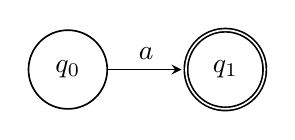
\begin{tikzpicture}[
    > = stealth,
    shorten > = 1pt,
    auto,
    node distance = 2cm,
    semithick,
    state/.style={circle, draw, minimum size=1cm}
]
    \node[state] (q0) {$q_0$};
    \node[state, accepting, right of=q0] (q1) {$q_1$};
    
    \path[->] (q0) edge node {$a$} (q1);
\end{tikzpicture}
\caption{NFA for single character $a$}
\end{figure}

\textbf{Concatenation} $AB$:

\begin{figure}[h!]
\centering
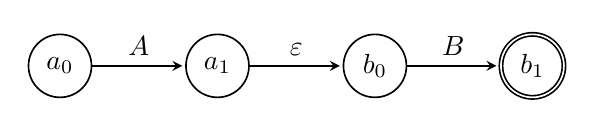
\begin{tikzpicture}[
    > = stealth,
    shorten > = 1pt,
    auto,
    node distance = 2cm,
    semithick,
    state/.style={circle, draw, minimum size=0.8cm}
]
    \node[state] (a0) {$a_0$};
    \node[state, right of=a0] (a1) {$a_1$};
    \node[state, right of=a1] (b0) {$b_0$};
    \node[state, accepting, right of=b0] (b1) {$b_1$};
    
    \path[->] 
        (a0) edge node {$A$} (a1)
        (a1) edge node {$\varepsilon$} (b0)
        (b0) edge node {$B$} (b1);
\end{tikzpicture}
\caption{NFA for concatenation $AB$}
\end{figure}

\textbf{Alternation} $A|B$:

\begin{figure}[h!]
\centering
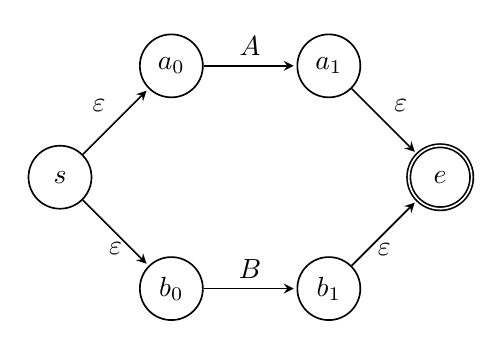
\begin{tikzpicture}[
    > = stealth,
    shorten > = 1pt,
    auto,
    node distance = 2cm,
    semithick,
    state/.style={circle, draw, minimum size=0.8cm}
]
    \node[state] (start) {$s$};
    \node[state, above right of=start] (a0) {$a_0$};
    \node[state, right of=a0] (a1) {$a_1$};
    \node[state, below right of=start] (b0) {$b_0$};
    \node[state, right of=b0] (b1) {$b_1$};
    \node[state, accepting, below right of=a1] (end) {$e$};
    
    \path[->]
        (start) edge node {$\varepsilon$} (a0)
        (start) edge node[below] {$\varepsilon$} (b0)
        (a0) edge node {$A$} (a1)
        (b0) edge node {$B$} (b1)
        (a1) edge node {$\varepsilon$} (end)
        (b1) edge node[below] {$\varepsilon$} (end);
\end{tikzpicture}
\caption{NFA for alternation $A|B$}
\end{figure}

\textbf{Kleene Star} $A*$:

\begin{figure}[h!]
\centering
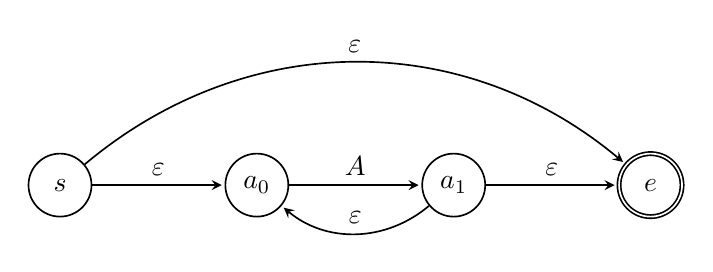
\begin{tikzpicture}[
    > = stealth,
    shorten > = 1pt,
    auto,
    node distance = 2.5cm,
    semithick,
    state/.style={circle, draw, minimum size=0.8cm}
]
    \node[state] (start) {$s$};
    \node[state, right of=start] (a0) {$a_0$};
    \node[state, right of=a0] (a1) {$a_1$};
    \node[state, accepting, right of=a1] (end) {$e$};
    
    \path[->]
        (start) edge node {$\varepsilon$} (a0)
        (a0) edge node {$A$} (a1)
        (a1) edge node {$\varepsilon$} (end)
        (start) edge[bend left=40] node[above] {$\varepsilon$} (end)
        (a1) edge[bend left=40] node[above] {$\varepsilon$} (a0);
\end{tikzpicture}
\caption{NFA for Kleene star $A*$}
\end{figure}

\subsection{Subset Construction (NFA to DFA)}

\textbf{Algorithm:}

\begin{enumerate}
    \item Start with $\varepsilon$-closure of NFA start state
    \item For each DFA state $D$ and input symbol $a$:
        \begin{itemize}
            \item Find all NFA states reachable from $D$ on $a$
            \item Take $\varepsilon$-closure of result
            \item This forms new DFA state
        \end{itemize}
    \item Mark DFA states containing NFA accepting states as accepting
    \item Repeat until no new states created
\end{enumerate}

\textbf{Example:} Pattern \texttt{[0-9]+}

\textbf{NFA:}
\[
q_0 \xrightarrow{[0-9]} q_1 \xrightarrow{\varepsilon} q_0 \quad \text{and} \quad q_1 \text{ is accepting}
\]

\textbf{DFA (after subset construction):}
\[
q_0 \xrightarrow{[0-9]} q_1 \quad \text{and} \quad q_1 \xrightarrow{[0-9]} q_1 \quad \text{(self-loop)}
\]

\subsection{DFA Minimization}

\textbf{Goal:} Reduce number of states while preserving language

\textbf{Algorithm (Hopcroft's):}
\begin{enumerate}
    \item Partition states into accepting and non-accepting
    \item Refine partitions iteratively:
        \begin{itemize}
            \item Split partitions where states differ in transitions
            \item Continue until no more splits possible
        \end{itemize}
    \item Merge states in same partition
\end{enumerate}

\section{Flex Specification Structure}

\subsection{Definitions Section}

\begin{lstlisting}[language=Lex]
%{
#include <stdio.h>
#include "tok_def.h"

int line_number = 1;
int error_count = 0;
%}

digit [0-9]
letter [a-zA-Z_]
alphanum [a-zA-Z0-9_]
\end{lstlisting}

\textbf{Components:}
\begin{itemize}
    \item C code in \texttt{\%\{ \%\}} blocks
    \item Pattern name definitions
    \item Options (e.g., \texttt{\%option yylineno})
\end{itemize}

\subsection{Rules Section}

\begin{lstlisting}[language=Lex]
%%
"<<"                { return BIT_LSHIFT_TOK; }
">>"                { return BIT_RSHIFT_TOK; }
{letter}{alphanum}* { return check_keyword(yytext); }
{digit}+            { return INTCONST_TOK; }
[ \t]+              { /* skip whitespace */ }
\n                  { line_number++; }
.                   { return ERROR; }
%%
\end{lstlisting}

\textbf{Pattern-Action Pairs:}
\begin{itemize}
    \item Pattern: Regular expression to match
    \item Action: C code to execute when matched
    \item Priority: First match wins if equal length
\end{itemize}

\subsection{User Code Section}

\begin{lstlisting}[language=C]
int main(int argc, char **argv) {
    if (argc > 1)
        yyin = fopen(argv[1], "r");
    
    int token;
    while ((token = yylex()) != 0) {
        printf("Token: %d\n", token);
    }
    
    return 0;
}
\end{lstlisting}

\section{Pattern Matching Details}

\subsection{Regular Expression Operators}

\begin{table}[h!]
\centering
\begin{tabularx}{\textwidth}{|l|l|X|}
\hline
\textbf{Operator} & \textbf{Example} & \textbf{Meaning} \\
\hline
\texttt{.} & \texttt{a.b} & Any character between a and b \\
\hline
\texttt{*} & \texttt{a*} & Zero or more a's \\
\hline
\texttt{+} & \texttt{a+} & One or more a's \\
\hline
\texttt{?} & \texttt{a?} & Zero or one a \\
\hline
\texttt{|} & \texttt{a|b} & a or b \\
\hline
\texttt{[]} & \texttt{[abc]} & Character class: a, b, or c \\
\hline
\texttt{[\^{}]} & \texttt{[\^{}abc]} & Negated class: not a, b, or c \\
\hline
\texttt{\{\}} & \texttt{a\{2,4\}} & 2 to 4 a's \\
\hline
\texttt{()} & \texttt{(ab)+} & Grouping \\
\hline
\end{tabularx}
\caption{Flex Regular Expression Operators}
\end{table}

\subsection{Character Classes}

\textbf{Predefined (with \texttt{[:...:]}))}:
\begin{itemize}
    \item \texttt{[:digit:]} = \texttt{[0-9]}
    \item \texttt{[:alpha:]} = \texttt{[a-zA-Z]}
    \item \texttt{[:alnum:]} = \texttt{[a-zA-Z0-9]}
    \item \texttt{[:space:]} = whitespace characters
\end{itemize}

\textbf{Custom Definitions:}
\begin{lstlisting}[language=Lex]
digit [0-9]
letter [a-zA-Z_]
id {letter}({letter}|{digit})*
\end{lstlisting}

\subsection{Maximal Munch Principle}

\textbf{Definition:} Always match the longest possible token

\textbf{Example:}
\begin{lstlisting}[language=Lex]
"<<"    { return LSHIFT; }
"<"     { return LESS; }
\end{lstlisting}

Input \texttt{<<} matches \texttt{LSHIFT}, not two \texttt{LESS} tokens.

\section{Generated Code Structure}

\subsection{yylex() Function}

Flex generates the \texttt{yylex()} function:

\begin{lstlisting}[language=C]
int yylex(void) {
    int state = 0;
    
    while (1) {
        int c = input();
        
        // State transitions based on DFA
        state = yy_next_state[state][c];
        
        if (is_accepting_state(state)) {
            // Execute action for matched pattern
            return token_type;
        }
        
        if (is_error_state(state)) {
            // Handle error
        }
    }
}
\end{lstlisting}

\subsection{Global Variables}

\begin{itemize}
    \item \texttt{char *yytext}: Current token text
    \item \texttt{int yyleng}: Length of current token
    \item \texttt{int yylineno}: Current line number
    \item \texttt{FILE *yyin}: Input file pointer
    \item \texttt{FILE *yyout}: Output file pointer
\end{itemize}

\subsection{Optimization Techniques}

Flex applies several optimizations:
\begin{enumerate}
    \item \textbf{Direct-coded DFA}: No table lookup overhead
    \item \textbf{Compressed tables}: Reduce memory usage
    \item \textbf{Fast character classification}: Bit operations
    \item \textbf{Inlined actions}: Reduce function call overhead
\end{enumerate}

\section{Integration with Parser}

\subsection{Token Communication}

\textbf{Lex side:}
\begin{lstlisting}[language=Lex]
%{
#include "parser.tab.h"  // Token definitions from Yacc
%}

%%
"int"       { return INT_TOK; }
[a-zA-Z_]+  { yylval.sval = strdup(yytext); return ID_TOK; }
[0-9]+      { yylval.ival = atoi(yytext); return INTCONST_TOK; }
%%
\end{lstlisting}

\textbf{Yacc side:}
\begin{lstlisting}[language=C]
%union {
    int ival;
    char *sval;
}

%token <sval> ID_TOK
%token <ival> INTCONST_TOK
%token INT_TOK
\end{lstlisting}

\subsection{Token Flow}

\begin{figure}[h!]
\centering
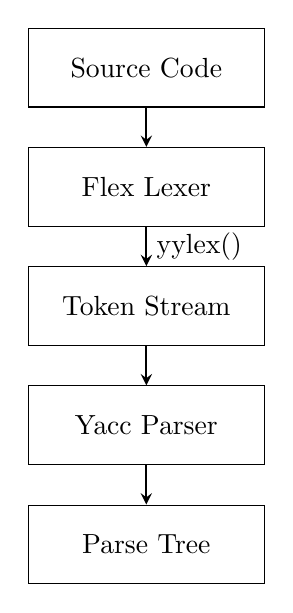
\begin{tikzpicture}[
    box/.style={rectangle, draw, minimum width=3cm, minimum height=1cm},
    arrow/.style={->, >=stealth, thick}
]
    \node[box] (source) {Source Code};
    \node[box, below=0.5cm of source] (lex) {Flex Lexer};
    \node[box, below=0.5cm of lex] (tokens) {Token Stream};
    \node[box, below=0.5cm of tokens] (yacc) {Yacc Parser};
    \node[box, below=0.5cm of yacc] (tree) {Parse Tree};
    
    \draw[arrow] (source) -- (lex);
    \draw[arrow] (lex) -- node[right] {yylex()} (tokens);
    \draw[arrow] (tokens) -- (yacc);
    \draw[arrow] (yacc) -- (tree);
\end{tikzpicture}
\caption{Lexer-Parser Communication}
\end{figure}

\section{Error Handling}

\subsection{Lexical Error Detection}

\begin{lstlisting}[language=Lex]
.   {
    printf("Invalid character: '%c' at line %d\n", 
           yytext[0], yylineno);
    error_count++;
}
\end{lstlisting}

\textbf{Strategy:} Catch-all pattern \texttt{.} at end of rules

\subsection{Spelling Error Detection}

Custom error checking (Assignment 02 v1 feature):

\begin{lstlisting}[language=C]
int check_spelling_error(char* word) {
    char* keywords[] = {"int", "float", "char", ...};
    char* errors[] = {"itn", "flot", "chr", ...};
    
    for (int i = 0; i < num_keywords; i++) {
        if (strcmp(word, errors[i]) == 0) {
            printf("SPELLING ERROR: '%s' - "
                   "Did you mean '%s'?\n",
                   word, keywords[i]);
            return 1;
        }
    }
    return 0;
}
\end{lstlisting}

\section{Performance Analysis}

\subsection{Time Complexity}

\textbf{DFA Simulation:} $O(n)$ where $n$ = input length
\begin{itemize}
    \item Each character examined once
    \item Constant time per state transition
    \item No backtracking required
\end{itemize}

\subsection{Space Complexity}

\textbf{DFA Storage:} $O(s \times |\Sigma|)$ where $s$ = states, $|\Sigma|$ = alphabet size
\begin{itemize}
    \item Transition table dominates space
    \item Compression reduces memory usage
    \item Token buffer: $O(k)$ for max token length $k$
\end{itemize}

\subsection{Comparison}

\begin{table}[h!]
\centering
\begin{tabular}{|l|c|c|}
\hline
\textbf{Metric} & \textbf{Hand-Written} & \textbf{Flex} \\
\hline
Time Complexity & $O(n)$ & $O(n)$ \\
Space Complexity & $O(k)$ & $O(s \times |\Sigma|)$ \\
Development Time & High & Low \\
Performance & Variable & Optimized \\
\hline
\end{tabular}
\caption{Performance Comparison}
\end{table}

\section{Summary}

This Flex-based lexical analyzer demonstrates:

\begin{enumerate}
    \item \textbf{Automated Generation}: From patterns to optimized code
    \item \textbf{Regular Expression Theory}: Thompson's construction and subset algorithm
    \item \textbf{DFA Optimization}: Minimization for efficiency
    \item \textbf{Standard Interface}: yylex, yytext conventions
    \item \textbf{Parser Integration}: Seamless token communication
    \item \textbf{Error Handling}: Lexical and spelling error detection
\end{enumerate}

The implementation shows how theoretical concepts (RE, NFA, DFA) translate to practical, efficient scanners through automated tools.

\section{References}

\begin{itemize}
    \item Levine, J.R. (2009). \emph{flex \& bison}. O'Reilly Media.
    \item Aho, A.V., Lam, M.S., Sethi, R., \& Ullman, J.D. (2006). \emph{Compilers: Principles, Techniques, and Tools} (2nd ed.).
    \item Hopcroft, J.E., Motwani, R., \& Ullman, J.D. (2006). \emph{Introduction to Automata Theory, Languages, and Computation} (3rd ed.).
    \item Flex Manual: \url{https://westes.github.io/flex/manual/}
\end{itemize}

\end{document}
